\documentclass[border=3pt]{standalone}
\usepackage{tikz}
\usetikzlibrary{arrows.meta,calc,positioning}
\tikzset{pin/.style={-{Stealth[length=5pt]}},
  blk/.style={draw, thick, font=\sffamily\small, align=center}}
\begin{document}
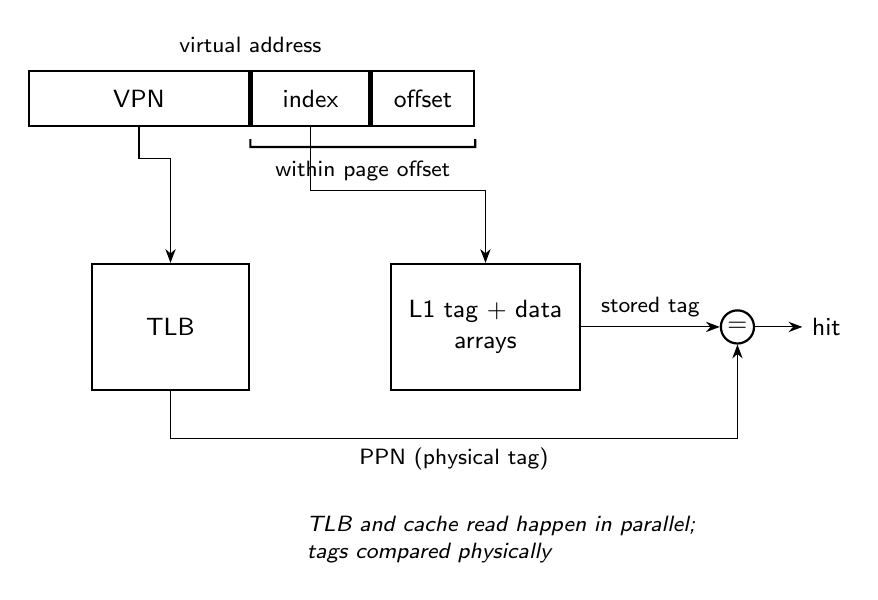
\begin{tikzpicture}[font=\sffamily\small]
  % VA fields
  \node[blk, minimum width=28mm, minimum height=7mm] (vpn) at (0,0) {VPN};
  \node[blk, minimum width=15mm, minimum height=7mm, anchor=west] (idx) at (vpn.east) {index};
  \node[blk, minimum width=13mm, minimum height=7mm, anchor=west] (off) at (idx.east) {offset};
  \node[font=\sffamily\footnotesize, above=1mm of vpn.north east] {virtual address};
  \draw [thick] ($(idx.south west)+(0,-1.5mm)$) -- ++(0,-1mm) -- node[below=0.5mm, font=\sffamily\footnotesize]{within page offset} ($(off.south east)+(0,-2.5mm)$) -- ++(0,1mm);
  % TLB
  \node[blk, minimum width=20mm, minimum height=16mm] (tlb) at (0.4,-2.9) {TLB};
  \draw[pin] (vpn.south) -- ++(0,-4mm) -| (tlb.north);
  % cache arrays
  \node[blk, minimum width=24mm, minimum height=16mm] (arr) at (4.4,-2.9) {L1 tag + data\\arrays};
  \draw[pin] (idx.south) -- ++(0,-8mm) -| (arr.north);
  % comparator
  \node[draw, thick, circle, inner sep=1.5pt] (cmp) at (7.6,-2.9) {$=$};
  \draw[pin] (tlb.south) |- node[below, font=\sffamily\footnotesize, pos=0.75]{PPN (physical tag)} ++(72mm,-6mm) -| (cmp.south);
  \draw[pin] (arr.east) -- node[above, font=\sffamily\footnotesize]{stored tag} (cmp.west);
  \draw[pin] (cmp.east) -- ++(6mm,0) node[right]{hit};
  \node[font=\sffamily\footnotesize\itshape, align=left] at (4.6,-5.6) {TLB and cache read happen in parallel;\\tags compared physically};
\end{tikzpicture}
\end{document}
